%KELOMPOK 2 Pemasukan
%\begin{enumerate}
%\item Imron Sumadireja
%\item Jesron Marudut Hatuan
%\item Lusia Violita
%\item Mhd Zulfikar Akram Nst
%\end{enumerate}

\section{Pengertian Flask}
\emph{Flask} adalah \emph{framework} aplikasi web mikro yang ditulis dalam bahasa Python dan berbasiskan \emph{toolkit Wekzeug} dan \emph{template engine Jinja2} dan berlisensi BSD. Flask dikatakan framework mikro dikarenakan Flask tidak menganggap atau mengharuskan pengembang komponen menggunakan alat atau pustaka tertentu. Flask tidak memiliki lapisan abstrak basis data, validasi form, dan komponen-komponen lainnya yang sudah dimiliki oleh pustaka-pustaka sebelumnya. Flask mendukung ekstensi yang dapat menambah fitur-fitur seperti layaknya mereka diimplmenetasikan di dalam Flask itu sendiri. Terdapat ekstensi untuk objek-relational mappers, validasi form, upload handlint, dan berbagai teknologi otentikasi terbuka serta peralatan yang berhubungan dengan framework secara umum\cite{solihin2016implementasi}.

\section{Pengertian Flask 2}
Flask adalah kerangka kerja mikro karena hanya mengimplementasikan fungsi inti (termasuk routing) tetapi meninggalkan fungsi yang lebih canggih (termasuk otentikasi dan datahase ORM) ekstensi. Hasil dari ini adalah pengaturan awal kurang untuk pengguna pertama kali dan lebih banyak pilihan dan fleksibilitas untuk pengguna yang berpengalaman. Hal ini berbeda dengan "kerangka kerja" yang lebih lengkap, seperti Django, yang menentukan teknologi ORM dan otentikasi mereka sendiri\cite{dwyer2016flask}.

\section{Fungsi Flask}
Flask berfungsi sebagai pengganti PHP POST dan GET yang dimana pengendali pertukaran data dari HTML ke database. Flask juga menggantikan fungsi Apache sebagai webserver dimana flask berjalan di http://localhost:5000/.
Flask dipilih karena berjalan diatas bahasa pemrograman Python sehingga lebih mudah diintegrasikan untuk mengontrol Virtual Data Center. Flask juga mengatur keluar masuknya data ke MySql untuk menyimpan inrformasi dan data dari user\cite{alauddin2017implementasi}.

\subsection{Fungsi Flask}
Flask juga mengolah data untuk ditampilkan ke web untuk mempermudah user dalam memahami data tersebut. Flask sendiri merupakan kerangka kerja berbasis bahasa pemograman python yang sangat cocok untuk diintegrasikan bersama aplikasi berbasis cloud. Selain berfungsi sebagai penghubung antar Virtual Data Center dan web, Flask juga bertanggung jawab atas pengintegrasian database yang dimana disini dipilih MySql sebagai database\cite{alauddin2017implementasi}.


\section{Fitur Flask}
Flask mendukung ekstensi. Ekstensi yang tersedia untuk objek relasional seperti pembuatan peta,
validasi formulir, upload handling, teknologi otentikasi, dan lain sebagainya. Berikut ini adalah beberapa
fitur yang dimiliki oleh flask, diantaranya :
\begin{enumerate}
  \item Integrated supports for unit testing
  \item Uses Jinja2 templating
  \item Support for secure cookies
  \item Extensive documentation
  \item Google app engine compatibility
  \item Restful request dispatching
  \item Unicode based\cite{lokhande2015efficient}.
\end{enumerate}

\section{Aplikasi dan Merekuest Konteks}
Ketika flask menerima permintaan dari klien, maka perlu membuat beberapa objek tersedia untuk fungsi tampilan yang akan menangani flasknya. Contoh yang baik adalah pada objek permintaan, yang merangkum permintaan HTTP yang dikirim oleh klien. Cara yang jelas di mana Flask bisa memberikan fungsi tampilan akses ke objek permintaan adalah dengan mengirimkannya sebagai argumen, tapi itu akan membutuhkan setiap fungsi tampilan tunggal dalam aplikasi untuk memiliki argumen tambahan\cite{grinberg2018flask}.

\subsection{Aplikasi dan Merekuest Konteks}
Hal-hal menjadi lebih rumit jika Anda menganggap bahwa objek permintaan bukan satu-satunya objek yang mungkin diperlukan fungsi tampilan untuk mengakses untuk memenuhi permintaan. Untuk menghindari fungsi tampilan yang kacau dengan banyak argumen yang mungkin tidak selalu diperlukan, Flask menggunakan konteks untuk sementara membuat objek tertentu dapat diakses secara global. Berkat konteksnya, lihat fungsi seperti follwing dapat ditulis:\cite{grinberg2018flask}.

\subsection{Aplikasi dan Merekuest Konteks}
\begin{verbatim}
from flask import request

@app.route('/')
def index():
	user_agent = request.headers.get('User-Agent')
	return '<p>Your browser is {}</p>'.format(user_agent)
\end{verbatim}
Perhatikan bagaimana dalam fungsi tampilan ini, permintaan digunakan seolah-olah itu adalah variabel global. Pada kenyataannya, permintaan tidak bisa menjadi variabel emas; di server multithread, beberapa utas dapat mengerjakan permintaan yang berbeda dari klien yang berbeda pada saat yang sama, sehingga setiap utas perlu melihat objek yang berbeda sesuai permintaan. Konteks memungkinkan Flask untuk membuat variabel tertentu yang dapat diakses secara global ke utas tanpa mengganggu benang yang lain\cite{grinberg2018flask}.

\subsection{Aplikasi dan Merekuest Konteks}
Catatan.
Thread adalah urutan instruksi terkecil yang dapat dikelola secara independen. Adalah umum untuk suatu proses untuk memiliki beberapa untaian aktif, terkadang berbagi sumber daya seperti memori atau menangani file. Beberapa untaian aktif, terkadang berbagi sumber daya seperti memori atau menangani file. Server web multithreaded memulai kumpulan benang dan memilih utas dari kolam untuk menangani setiap permintaan masuk\cite{grinberg2018flask}.

\section{Implementasi Flask Post - Python}
Untuk demonstrasi, aplikasi demo posting blog menyajikan implementasi praktis API. Aplikasi ini menggunakan kerangka web Flask-Python. Selain itu, bagian ini memperkenalkan teknologi yang digunakan dan menyebutkan alasan mengapa mereka dipilih untuk proyek tersebut. Selain itu, ia menyediakan langkah demi langkah pendekatan untuk menunjukkan bagaimana sumber daya dibagi dari sumber data persisten. Oleh karena itu, API aplikasi mendasarkan prinsip REST\cite{alemu2014rest}.

\subsection{Tiga Alasan memilih Flask untuk Aplikasi Demo}
Ada tiga alasan untuk memilih Flask untuk aplikasi demo ini.
\begin{enumerate}
\item Pertama salah satunya adalah kesederhanaannya.
\item Kedua adalah keterbukaannya.
\item Ketiga adalah open source yang terdokumentasi dengan baik kerangka.
\end{enumerate}
Dalam Flask, seseorang seharusnya tidak perlu tahu segalanya dari awal. Kerangka kerja bisa dipelajari sambil berkembang. Ini memiliki awal yang cepat dokumentasi yang memandu pengembang untuk membuka dan menjalankan aplikasi dengan dasar fungsionalitas. Seperti halnya Python, Flask perangkat lunak didistribusikan di bawah lisensi sumber terbuka permisif. Ini membuat lebih mudah diakses dan canggih.  Ini memiliki tutorial rinci selain dokumentasi mulai cepat. Selain itu, ia menyediakan dokumentasi terbaru untuk setiap versi baru kerangka. Oleh karena itu, alasan-alasan ini membuat kerangka web Flask lebih disukai aplikasi demo layanan web blogging\cite{alemu2014rest}.

\section{Kekurangan Flask}
Salah satu kekurangan dari Flask secara garis besar, Microframework berarti framework dengan skala kecil atau mikro, tidak semua fungsi dapat diimplementasikan di dalam Flask Microframework.  Di dalam Flask Microframework programmer di paksa untuk menulis syntaxnya sendiri mulai dari 0 atau kita dapat mengatakan kita membuat blog atau web kita mulai dari scratch. Dan juga tidak semua fungsi pada web pada umumnya dapat langsung diimplementasikan, seperti contohnya koneksi ke database, login function, dan lainnya\cite{ronacher2010flask}.

\section{Flask - HTTP Method POST}
Web Server dirancang untuk menanggapi permintaan GET HTTP dengan mengambil sumber daya yang cocok dengan kriteria query. Di URI (Uniform Resource Identifier) permintaan dan mengembalikan dalam response, bukan untuk menambahkan catatan pada database\cite{rodriguez2008restful}. Secara default flask hanya menangani permintaan GET. Jika perlu memproses jenis permintaan lainnya, harus memberikan metode atribut class berikut ini:

\begin{verbatim}
from flask.views import View

class MyRequest(View):
    methods = ['POST']

    def dispatch_request(self):
        # request.method == 'POST'
        name = request.form.get('name', 'Damyan')
        return 'Hello, %s!' % name

app.add_url_rule(
    '/say-hi', view_func=MyRequest.as_view('my_request')
)
\end{verbatim}

Dalam hal permintaan POST, bisa mengambil nilai yang diposting menggunakan metode request.form.get(). Metode dalam dispatch_request memberikan pemrosesan khusus untuk GET, dan permintaan POST. Disinilah MethodView digunakan:

\begin{verbatim}
from flask.views import MethodView

class GenericRequest(MethodView):
    def get(self):
        name = request.args.get('name', 'Damyan')
        return 'Hello GET from %s!' % name

    def post(self):
        name = request.form.get('name', 'Damyan')
        return 'Hello POST from %s' % name

app.add_url_rule(
    '/generic_request',
    view_func=GenericRequest.as_view('generic_request')
)
\end{verbatim}

\section{Flask API}
Flask API merupakan implementasi dari web API yang dapat dijelajahi menggunakan kerangka yang sudah disediakan Django REST. Django REST merupakan web framework sumber terbuka berbasis Python. Aplikasi web yang dibuat dengan Flask disimpan dalam satu berkas .py. Flask merupakan web framework yang sederhana namun dapat diperluas dengan beragam pustaka tambahan yang sesuai dengan kebutuhan penggunanya. Flask API menyimpan perintah-perintah dari gphoto library dan piggyphoto library\cite{computingaplikasi}.

\subsection{Fungsi Flask API}
Selain Flask merupakan web framework yang sederhana, Flask API berfungsi sebagai jembatan penghubung antara Raspberry Pi dan smartphone Android. Untuk mendapatkan micro framework Flask, kita harus install Flask API, Setelah instalasi Flask Micro Framework selesai dilanjutkan dengan mengatur perintah-perintah dari gphoto2 library dan piggyphoto pada Flask API agar dapat diakses melalui HTTP-Request\cite{computingaplikasi}.

\section{Flask Post Parsing JSON}
Tujuan dari posting ini adalah untuk menjelaskan cara mengurai dan menggunakan data JSON dari permintaan POST di Flask, kerangka web mikro untuk Python. Pertama-tama, kita perlu mengimpor kelas Flask dari modul flask, sehingga semua fungsi yang kita butuhkan tersedia. Kemudian,kita harus membuat instance kelas Flask. Asumsikan bahwa klien akan memposting data JSON, jadi tentukan rute yang hanya menjawab permintaan HTTP POST. Permintaan GET apa pun ke URL yang sama akan diabaikan\cite{dwyer2016flask}.

\subsection{Menentukan Kata Kunci POST}
Tentukan kata kunci POST ke argumen metode dekorator rute. Anda dapat membaca lebih lanjut tentang cara mengontrol metode yang diizinkan HTTP dalam posting. Perhatikan  bahwa server akan mendengarkan di URL / postjson.  Pertama, untuk mengonfirmasi apakah konten berjenis JSON. Atribut ini menunjukkan jika permintaan ini adalah JSON atau bukan . Untuk mendapatkan data JSON yang diposting, kita hanya perlu memanggil metode get_json pada objek permintaan, yang mem-parsing data permintaan JSON yang masuk dan mengembalikannya sebagai kamus Python\cite{dwyer2016flask}.

\section{Membuat JSON Menggunakan Python}
Logika dasar untuk membuat data JSON ialah membuat kamus dan menambahkannya ke daftar. Setelah menambahkan ke daftar selesai, selanjutnya akan mengonversi daftar menjadi data JSON. Berikut contoh script yang digunakan:
\begin{verbatim}
@app.route("/getLatihanList")
def getLatihanList():

    try:


        latihanList = []


        for i in range(0,2):
        empDict = {
        'firstName': 'Arya',
        'lastName': 'Santoso'}
            latihanList.append(empDict)


        jsonStr = json.dumps(latihanList)

    except Exception ,e:
        print str(e)

    return jsonify(Latihan=jsonStr)
\end{verbatim}
Dalam contoh kode diatas, cukup menggulirkan data dua kali dan membuat kamus kosong. Menggunakan json.dumps berfungsi untuk mengonversi dari kamus ke string JSON. Setelah itu lakukan running untuk menjalankan script diatas, jika berhasil maka akan seperti berikut ini:
\begin{verbatim}
{
    "Latihan": [{
        "firstName": "Arya",
        "lastName": "Santoso"
    }, {
        "firstName": "Arya",
        "lastName": "Santoso"
    }]
}
\end{verbatim}

\section{POST request using Python}
Perbedaan antara POST dan PUT ialah PUT merupakan idempoten, yakni memanggilnya hanya sekali atau beberapa kali berturut-turut memiliki efek yang sama (tidak ada efek samping), sedangkan POST identik dengan yang berurutan dan dapat memiliki efek tambahan, seperti melewatkan pesanan beberapa kali. Gambar \ref{3post} adalah diagram sederhana yang menjelaskan konsep dasar metode GET dan POST.

\begin{figure}[ht]
\centerline{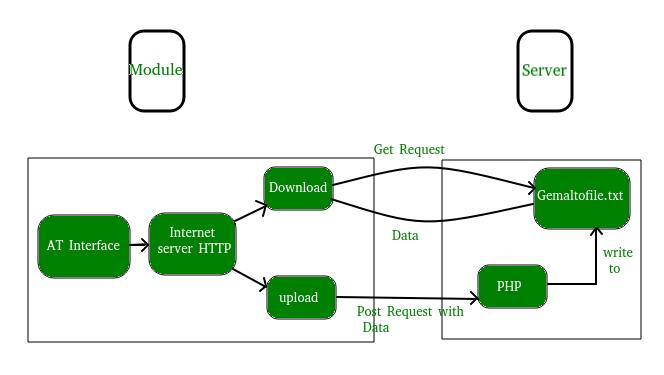
\includegraphics[width=1\textwidth]{figures/3post.png}}
\caption{Client Server}
\label{3post}
\end{figure}

Untuk POST, GET, PUT, dan DELETE biasanya sudah ditentukan oleh protokol secara langung. Dan idealnya, untuk menjaga interfaces umum dan memungkinkan klien untuk secara eksplisit tentang operasi yang mereka gunakan\cite{rodriguez2008restful}.

\section{Memproses Data Permintaan yang Masuk dalam Flask}
Di aplikasi web apa pun, Anda harus memproses data permintaan masuk dari pengguna. Flask, seperti kerangka web lainnya, memungkinkan Anda untuk mengakses data permintaan dengan mudah. Untuk mengakses data yang masuk dalam Flask, Anda harus menggunakan objek permintaan. Objek permintaan menampung semua data yang masuk dari permintaan, yang meliputi mimetype, referrer, alamat IP, data mentah, metode HTTP, dan header, dan sebagainya. Meskipun semua informasi yang dipegang oleh objek permintaan dapat berguna\cite{walsh2007application}.

\section{Transfer XML, JSON using Python}
Representasi biasanya mencerminkan keadaan resource saat ini, dan atributnya, pada waktu aplikasi klien memintanya. Representasi resource dalam pengertian ini hanyalah snapshot. Ini bisa menjadi hal yang sederhana seperti representasi catatan dalam database yang terdiri dari pemetaan antara nama kolom dan tag XML, di mana nilai elemen dalam XML mengandung nilai baris. Atau, jika sistem memiliki model data, maka menurut definisi ini resource representasi adalah snapshot dari atribut salah satu hal dalam model data sistem. Kumpulan kendala terakhir yang masuk ke desain layanan Web RESTEN ada hubungannya dengan format data yang aplikasi dan pertukaran layanan dalam permintaan / respons payload atau di HTTP\cite{rodriguez2008restful}.
